\begin{multicols}{2}
    

%%%%%%%%%%%%%%%%%%%%%%%%%%%%%%%%%%%%%%%%%%%%%%%%%%%%%%%%%%%%%%
% EJERCICIO 1
%%%%%%%%%%%%%%%%%%%%%%%%%%%%%%%%%%%%%%%%%%%%%%%%%%%%%%%%%%%%%%

\title{Diagnóstico de Cáncer de Mama: Análisis Exploratorio y Modelado Predictivo}
%%%%%%%%%%%%%%%%%%%%%%%%%%%%%%%%%%%%%%%%%%%%%%%%%%%%%%%%%%%%%%
\begin{abstract}
Este trabajo aborda el diagnóstico de cáncer de mama a partir de variables morfológicas y bioquímicas extraídas de imágenes histopatológicas, mediante un enfoque de análisis exploratorio y modelado predictivo. Se identificaron y trataron anomalías estructurales en los datos, como valores atípicos y ausencias, empleando técnicas de imputación por K-Nearest Neighbors y winsorización. Se desarrollaron modelos de regresión logística regularizada sobre conjuntos balanceados y desbalanceados, evaluando distintas estrategias de re-balanceo: \emph{oversampling}, \emph{undersampling}, \emph{SMOTE} y \emph{cost re-weighting}. 

En el caso de los datos balanceados, el modelo final alcanzó un recall de 0,8916, una precisión de 0,9250 y un F1-score de 0,9080 al ser evaluado sobre el conjunto de prueba, demostrando una excelente capacidad de generalización. Por su parte, el mejor resultado sobre el conjunto desbalanceado se obtuvo con \emph{cost re-weighting}, logrando un recall de 0,9118 y un AUC-PR de 0,8785. Estos resultados evidencian la solidez de los modelos propuestos en distintos escenarios clínicos.
\end{abstract}




%%%%%%%%%%%%%%%%%%%%%%%%%%%%%%%%%%%%%%%%%%%%%%%%%%%%%%%%%%%%%%
\section{Introducción}
El diagnóstico precoz del cáncer de mama resulta fundamental para mejorar las tasas de supervivencia y optimizar los tratamientos clínicos. En este trabajo se estudia un conjunto de datos derivados de imágenes histopatológicas de biopsias mamarias, del cual se extrajeron variables morfológicas y moleculares. El objetivo principal consiste en construir un modelo predictivo capaz de clasificar células como benignas (0) o malignas (1), a partir de 12 variables numéricas (como el tamaño celular, densidad nuclear o tasa mitótica) y 2 variables categóricas (tipo celular y presencia de mutaciones genéticas).
%%%%%%%%%%%%%%%%%%%%%%%%%%%%%%%%%%%%%%%%%%%%%%%%%%%%%%%%%%%%%%
\section{Metodología}
%%%%%%%%%%%%%%%%%%%%%%%%%%%%%%%%%%%%%%%%%%%%%%%%%%%%%%%%%%%%%%
\subsection{Preprocesamiento de Datos}

El preprocesamiento se realizó de manera diferenciada sobre dos versiones del conjunto de datos: una con clases balanceadas y otra con clases desbalanceadas. En ambos casos, los datos fueron divididos en conjuntos de entrenamiento (80\%) y validación (20\%), reservando un conjunto independiente para prueba. Se aplicaron técnicas de imputación de valores faltantes y tratamiento de outliers. Además, para el conjunto balanceado se generaron nuevas variables derivadas, mientras que para el conjunto desbalanceado se evaluaron distintas estrategias de re-balanceo durante la etapa de modelado.

\subsubsection{Conjunto de Datos Balanceado}
\label{subsec:preproc-balanced}

El conjunto balanceado presentó una distribución equitativa de la variable objetivo \texttt{Diagnosis}, con un 53{,}79\% de observaciones en la clase 0 y un 46{,}21\% en la clase 1. Esta condición permitió desarrollar modelos sin aplicar técnicas de re-balanceo.

En la etapa inicial se detectaron valores faltantes en 13 de las 14 variables predictoras. Aproximadamente el 92,26\% de las muestras presentaban al menos un valor ausente. Para su tratamiento, se aplicó imputación mediante el algoritmo de vecinos más cercanos (\textit{K-Nearest Neighbors}), con \(k = 8\) y distancia euclidiana como métrica, según el procedimiento detallado en el Apéndice~\ref{subsec:knn}. El 7,74\% restante de observaciones completas sirvió como base de referencia para esta imputación.

Posteriormente, se identificaron valores atípicos utilizando el método del rango intercuartílico (IQR), como se describe en el Apéndice~\ref{subsec:iqr}. Los valores extremos fueron corregidos mediante winsorización, ajustándolos al límite correspondiente según el rango definido por los cuartiles. Este procedimiento permitió reducir el impacto de outliers sin eliminar observaciones del conjunto.


A continuación, se analizaron las distribuciones de estas variables numéricas tras el preprocesamiento. La Figura~\ref{fig:distribution-fig} ilustra cómo dichas variables adoptan un comportamiento más simétrico y adecuado para su uso en modelos estadísticos.

\begin{figure}[H]
    \centering
    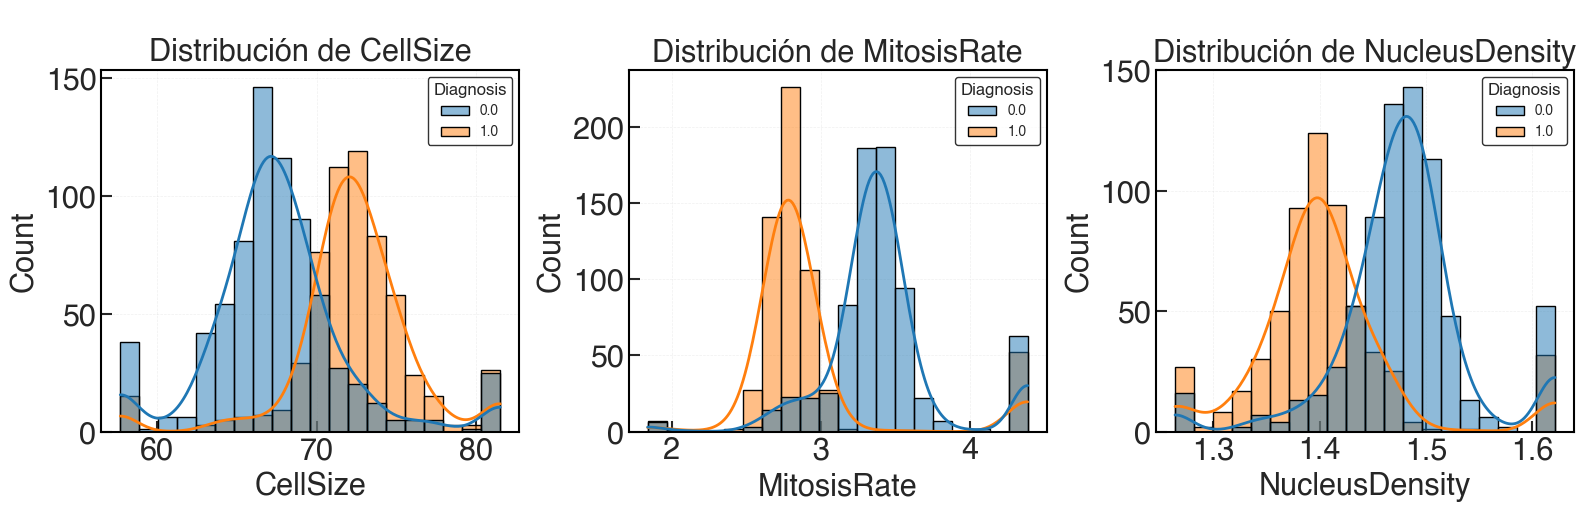
\includegraphics[width=1\linewidth]{figures/p1/numerical_distributions_outliers_balanced.png}
    \caption{Distribuciones de \texttt{CellSize}, \texttt{MitosisRate} y \texttt{NucleusDensity} tras el preprocesamiento (conjunto balanceado).}
    \label{fig:distribution-fig}
\end{figure}


Posteriormente, se evaluaron las correlaciones entre las variables numéricas y la variable objetivo \texttt{Diagnosis}, utilizando el coeficiente de Pearson. A diferencia del conjunto original, las características mostraron una asociación más clara luego del preprocesamiento, con coeficientes de correlación que oscilaron entre aproximadamente $-0.60$ y $0.63$. Esta mejora facilitó el análisis posterior y la selección de predictores relevantes.

Las variables categóricas fueron codificadas mediante \textit{One-Hot Encoding}, y las variables numéricas normalizadas en los casos que así lo requerían. Finalmente, se incorporaron variables derivadas mediante técnicas de \textit{feature engineering}, con el objetivo de enriquecer el conjunto de predictores:

\begin{itemize}
    \item Índice núcleo-citoplasma: \((\mathrm{CellSize} - \mathrm{CytoplasmSize}) / \mathrm{CytoplasmSize}\),
    \item Índice de proliferación celular: \(\mathrm{GrowthFactor} \times \mathrm{MitosisRate}\),
    \item Densidad nuclear: \(\mathrm{NucleusDensity} \times \mathrm{ChromatinTexture}\).
\end{itemize}


\subsubsection{Conjunto de Datos Desbalanceado}
\label{subsec:preproc-imbalanced}

En el conjunto desbalanceado, la variable \texttt{Diagnosis} presentó un desequilibrio considerable, con un 75\% de observaciones en la clase 0 y un 25\% en la clase 1. Debido a esta asimetría, se evaluaron distintas técnicas de re-balanceo (ver Apéndice~\ref{subsec:desbalanceo}) durante la etapa de modelado, pero el preprocesamiento estructural fue equivalente al aplicado sobre los datos balanceados (sección \ref{subsec:preproc-balanced}).

A diferencia del conjunto balanceado, en este caso no se aplicó \textit{feature engineering}, con el objetivo de aislar el impacto de las distintas técnicas de re-balanceo sobre el rendimiento del modelo. Para evaluar la calidad de las distribuciones numéricas obtenidas, se generaron visualizaciones análogas a las del conjunto balanceado. La Figura~\ref{fig:enter-label} muestra las nuevas distribuciones de las variables \texttt{CellSize}, \texttt{MitosisRate} y \texttt{NucleusDensity} tras el tratamiento de valores faltantes y atípicos.


\begin{figure}[H]
    \centering
    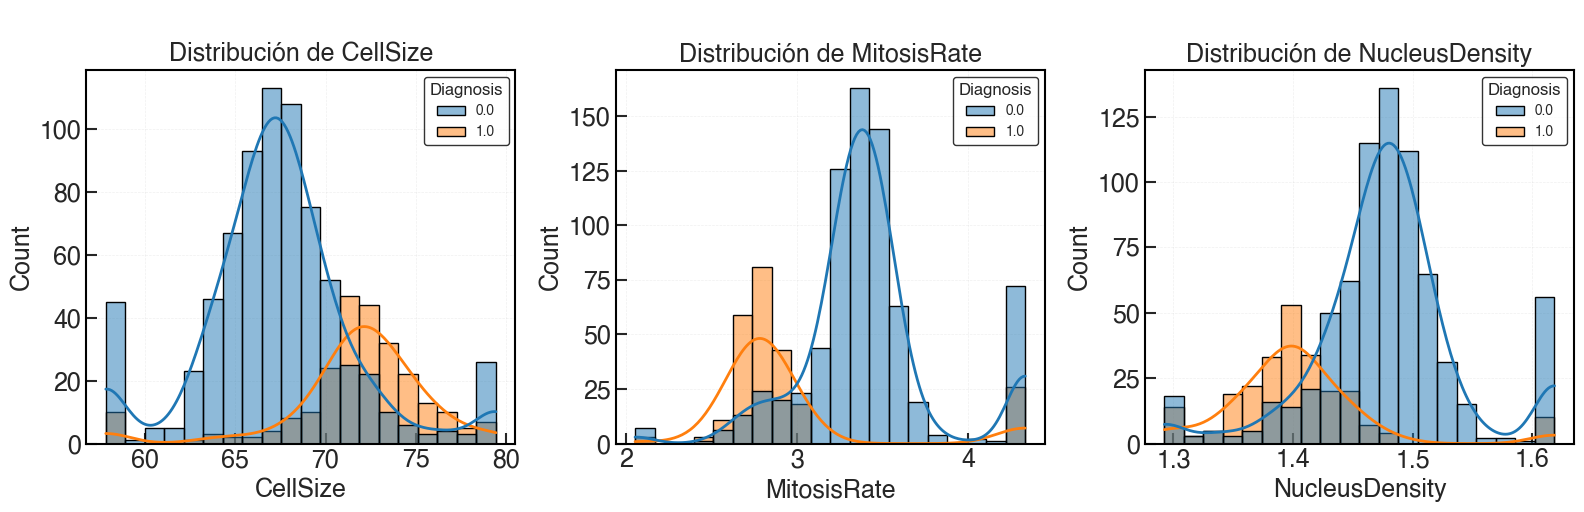
\includegraphics[width=1\linewidth]{figures/p1/distribucion_desbalanceados.png}
    \caption{Distribuciones de \texttt{CellSize}, \texttt{MitosisRate} y \texttt{NucleusDensity} tras el preprocesamiento (conjunto desbalanceado).}
    \label{fig:enter-label}
\end{figure}

Las correlaciones observadas entre las variables predictoras y la variable objetivo fueron consistentes con las obtenidas en el conjunto balanceado. Las pequeñas diferencias numéricas no afectaron las asociaciones estructurales principales, confirmando la estabilidad de los patrones estadísticos entre ambos conjuntos.

%%%%%%%%%%%%%%%%%%%%%%%%%%%%%%%%%%%%%%%%%%%%%%%%%%%%%%%%%%%%%%
\section{Resultados}
A continuación se presentan los principales resultados obtenidos tras la implementación y evaluación de distintas técnicas aplicadas a un modelo de Regresión Logística. Para una descripción detallada del proceso de entrenamiento, ajuste de hiperparámetros, métricas de desempeño  y técnicas de rebalanceo, se remite al Apéndice~\ref{subsec:modelado-predictivo},  Apéndice~\ref{subsec:desbalanceo}, Apéndice \ref{subsec:hiperparams-cancer} y Apéndice \ref{subsec:metricas-desempenio}, respectivamente.



\subsection{Datos Balanceados}

El desempeño del modelo fue inicialmente evaluado utilizando el conjunto de validación, lo que permitió obtener una primera estimación de su capacidad predictiva. Posteriormente, se procedió al reentrenamiento del modelo empleando la totalidad del conjunto de desarrollo, aplicando el preprocesamiento desde cero para evitar cualquier tipo de filtración de información y asegurar consistencia con el pipeline original, con el objetivo de aprovechar al máximo la información disponible antes de su evaluación final. Cabe señalar que, si bien el conjunto de validación cumple un rol clave en la comparación y selección entre múltiples modelos o configuraciones, en este caso particular —al tratarse de un único modelo base— se priorizó el análisis sobre el conjunto de prueba como instancia definitiva de evaluación del rendimiento.


En esta etapa se observó una mejora generalizada en las métricas, particularmente en la precisión, que alcanzó el 0,9259. El recall se mantuvo elevado (0{,}9036) y el F1 score fue de 0{,}9146, evidenciando un buen equilibrio entre Precision y Recall. La Tabla~\ref{tab:metrics_balanced} resume el rendimiento del modelo en ambas fases.

La Figura~\ref{fig:roc_auc_balanced_test} presenta la curva ROC obtenida sobre el conjunto de prueba, la cual permite visualizar la capacidad discriminativa del modelo frente a distintos umbrales de decisión. Junto con ella, se incorporan la matriz de confusión y la curva Precision-Recall, que complementan el análisis y permiten una evaluación más detallada del desempeño en cada clase. Estos resultados indican que el modelo es capaz de generalizar adecuadamente cuando se entrena sobre datos con distribución equilibrada, sin necesidad de aplicar técnicas adicionales de manejo de desbalanceo.

\subsection{Datos Desbalanceados}

En esta etapa se evaluó el impacto de distintas técnicas de re-balanceo aplicadas al conjunto de entrenamiento desbalanceado, utilizando validación cruzada para obtener métricas de rendimiento comparables. 

\subsubsection{Evaluación sobre el Conjunto de Validación}

Los resultados obtenidos en la validación muestran un desempeño general sólido para todas las estrategias evaluadas (ver Tabla~\ref{tab:val-metrics-imbalanced}). Sin embargo, dado el carácter clínico del problema —donde minimizar los falsos negativos es prioritario—, el foco se centró en la capacidad de los modelos para identificar correctamente la clase positiva. En este contexto, el recall se estableció como métrica principal, y se observó una mejora considerable en dicha métrica en todos los enfoques con re-balanceo respecto al modelo base.

Entre las técnicas aplicadas, \textit{SMOTE} y \textit{cost reweighting} se destacaron por ofrecer un alto nivel de recuperación de la clase positiva sin sacrificar significativamente otras métricas como la precisión o el F1-score. En particular, \textit{cost reweighting} obtuvo el mayor AUC-PR, lo que refuerza su eficacia en escenarios desbalanceados. Aunque el oversampling tradicional también alcanzó buen recall, su baja precisión sugiere una mayor proporción de falsos positivos, lo cual puede ser perjudicial en contextos clínicos. Por esta razón, \textit{cost reweighting} surge como la opción más equilibrada y recomendable.


\subsubsection{Evaluación sobre el Conjunto de Prueba}

Si bien el conjunto de prueba debe reservarse idealmente para la evaluación final del modelo seleccionado, en este trabajo se utilizó también con fines exploratorios, con el objetivo de comparar el desempeño general de cada técnica de re-balanceo en un entorno no visto durante el entrenamiento ni la validación. Esto permite observar la robustez de cada enfoque frente a nuevos datos y extraer conclusiones más informadas sobre su aplicabilidad en contextos reales.

Como se observa en la Tabla~\ref{tab:test-metrics-imbalanced}, y tal como se anticipaba a partir de los resultados en el conjunto de validación, la técnica de \textit{cost re-weighting} logró el mejor equilibrio general entre las métricas evaluadas. Por otro lado, en la Figura \ref{fig:roc_auc_imbalanced_test} se observan las curvas ROC y PR de los modelos entrenados con las diferentes técnicas de rebalanceo. Se observa que, además de mantener un recall elevado, obtuvo el mayor AUC-PR (0,8785), lo que refleja una notable capacidad para discriminar correctamente la clase minoritaria en un contexto desbalanceado.  A diferencia del \textit{oversampling}, que puede inducir sobreajuste al replicar instancias, el \textit{reweighting} ajusta la función de pérdida sin modificar la distribución original de los datos, preservando así la diversidad del conjunto de entrenamiento.

\subsubsection{Elección del modelo final}

De acuerdo con el criterio clínico adoptado, se priorizó el recall como métrica principal a la hora de elegir un modelo final. En línea con esta decisión, el modelo basado en \textit{cost re-weighting} resultó ser el más adecuado. El modelo final fue reentrenado sobre el conjunto completo de desarrollo, manteniendo el esquema de preprocesamiento y ajustando el hiperparámetro de regularización mediante validación cruzada con un valor óptimo de \(\lambda = 4.2813\).

La evaluación final del modelo sobre el conjunto de prueba evidenció un rendimiento consistente, con una accuracy de 0,9265, una precisión de 0,8158, un recall de 0,9118 y un F1-score de 0,8611. Estos resultados reflejan un buen equilibrio entre sensibilidad y precisión, y, lo más relevante, una sólida capacidad para identificar correctamente la clase minoritaria, aspecto crucial en tareas de diagnóstico clínico. La Figura~\ref{fig:metric_plot_imbalanced_cw} complementa estos resultados mediante la representación gráfica de la matriz de confusión, la curva ROC y la curva precision-recall, ofreciendo una visión más detallada del comportamiento del modelo frente a diferentes umbrales de decisión. Estos resultados reafirman que el modelo seleccionado ofrece un desempeño robusto y equilibrado, con excelente capacidad de generalización frente a datos desbalanceados, sin requerir la generación ni eliminación de observaciones artificiales.


\section{Conclusiones}

Este trabajo abordó el desafío del diagnóstico automatizado de cáncer de mama mediante un pipeline integral que incluyó análisis exploratorio, limpieza avanzada de datos y entrenamiento de modelos de clasificación. El preprocesamiento —que comprendió imputación con KNN, tratamiento de outliers y generación de variables derivadas— mejoró notablemente la calidad del conjunto de entrenamiento y permitió identificar relaciones más claras entre las variables predictoras y la clase objetivo, lo cual favoreció la construcción de modelos más eficientes y con mayor poder explicativo.

Frente al desbalance de clases, se compararon distintas estrategias, destacándose \textit{cost re-weighting} por su capacidad para mantener un alto nivel de recall sin alterar la distribución original de los datos. Esta técnica resultó ser la más adecuada para el contexto clínico planteado, donde los falsos negativos tienen un costo elevado. El modelo final, evaluado sobre un conjunto independiente, alcanzó un recall de 0.9118 y un AUC-PR de 0.8785, evidenciando su robustez y utilidad práctica en escenarios reales de diagnóstico médico.


\end{multicols}






